\documentclass[12pt, a4paper, onecolumn]{exam}

% Imports
\usepackage{amsmath}
\usepackage{amssymb}
\usepackage[lmargin=71pt, tmargin=1.2in]{geometry}  %For centering solution box
\usepackage{graphicx} % Required for inserting images
\usepackage{lastpage}
\usepackage{qrcode}
\usepackage{hyperref}
\usepackage{forest}
\usepackage{tikz}

% Document's meta-data
\newcommand{\subject}{Algorítimos e Estruturas de Dados Avançados}
\newcommand{\assignment}{Exercícios do Encontro 07}
\newcommand{\authorfullname}{José Augusto Queiroz Comparotto Gomes}
\newcommand{\authorname}{José A. Q. C. Gomes}
\newcommand{\authorno}{398439413098}
\newcommand{\professor}{Prof.ª Noiza Waltrick Trindade}
\newcommand{\course}{Ciência da Computação — Noturno}
\newcommand{\classno}{A}
\newcommand{\location}{Campo Grande-MS}
\newcommand{\documentdate}{Outubro de 2024}
\newcommand{\university}{Universidade Anhaguera — Uniderp}
\author{\authorfullname}
\title{\subject: \assignment}

% General page styling
\lhead{\subject\\}
\rhead{\assignment\\}
\lfoot{\authorname}
\cfoot{Página \thepage~de~\pageref{LastPage}}
\rfoot{RA:~\authorno}

\thispagestyle{empty}   %For removing header/footer from page 1

\begin{document}

% Forest default styling
\forestset{
  default tree style/.style={
    for tree = {circle, draw, minimum size=1.50em, inner sep=1pt, s sep=0.40cm}
  }
}

% Presenting page
\begingroup  

    \centering
    \begin{figure}
        \centering
        
\includegraphics[width=0.15\linewidth]{./assets/uniderp.jpg}\label{fig:university-logo}
    \end{figure}
    
    \rule{\textwidth}{2pt}  \\[1em]
    
    \LARGE \authorfullname\\
    \vfill
    \LARGE \subject\\
    \LARGE \assignment\\
    \vfill
    
    \large À \professor\\

    \vfill
    
    \large \course\\
    \large Turma \classno\\
    
    \rule{\textwidth}{2pt}\\[1em]

    \large \location\\
    \large \documentdate\\

    \pagebreak
\endgroup

\pointsdroppedatright%
\printanswers%
\renewcommand{\solutiontitle}{\noindent\textbf{Resposta:}\enspace}  

\begin{questions}
    
    % \question[q1] Inserir os elementos a seguir em uma árvore AVL, mostrando a árvore em cada etapa: 4, 5, 7, 2, 1, 3, 6.
    
    % \begin{solution}
        
    %     \centering
    %     \begin{minipage}{0.20\textwidth}
    %         \centering
    %         \begin{forest} default tree style
    %             [4]
    %         \end{forest}
    %     \end{minipage}
    %     \hfill
    %     \begin{tikzpicture}
    %         \draw[->] (0,0) -- (1.5,0) node[midway, above] {Inserção};
    %     \end{tikzpicture}
    %     \hfill
    %     \begin{minipage}{0.20\textwidth}
    %         \centering
    %         \begin{forest} default tree style
    %             [4
    %                 [, phantom]
    %                 [5, dotted]
    %             ]
    %         \end{forest}
    %     \end{minipage}
    %     \hfill
    %     \begin{tikzpicture}
    %         \draw[->] (0,0) -- (1.5,0) node[midway, above] {Inserção};
    %     \end{tikzpicture}
    %     \hfill
    %     \begin{minipage}{0.20\textwidth}
    %         \centering
    %         \begin{forest} default tree style
    %             [4
    %                 [, phantom]
    %                 [5
    %                     [, phantom]
    %                     [7, dotted]
    %                 ]
    %             ]
    %         \end{forest}
    %     \end{minipage}
        
    %     \begin{minipage}{0.25\textwidth}
    %         \centering
    %         \begin{forest} default tree style
    %             [4, red
    %                 [, phantom]
    %                 [5
    %                     [, phantom]
    %                     [7]
    %                 ]
    %             ]
    %         \end{forest}
    %     \end{minipage}
    %     \hfill
    %     \begin{tikzpicture}
    %         \draw[->] (0,0) -- (0.75,0) node[midway, above] {RR};
    %     \end{tikzpicture}
    %     \hfill
    %     \begin{minipage}{0.25\textwidth}
    %         \centering
    %         \begin{forest} default tree style
    %             [5
    %                 [4]
    %                 [7]
    %             ]
    %         \end{forest}
    %     \end{minipage}
    %     \hfill
    %     \begin{tikzpicture}
    %         \draw[->] (0,0) -- (1.5,0) node[midway, above] {Inserção};
    %     \end{tikzpicture}
    %     \hfill
    %     \begin{minipage}{0.25\textwidth}
    %         \centering
    %         \begin{forest} default tree style
    %             [5
    %                 [4
    %                     [2, dotted]
    %                     [, phantom]
    %                 ]
    %                 [7]
    %             ]
    %         \end{forest}
    %     \end{minipage}
        
    %      \begin{minipage}{0.30\textwidth}
    %         \centering
    %         \begin{forest} default tree style
    %             [5
    %                 [4
    %                     [2]
    %                     [, phantom]
    %                 ]
    %                 [7]
    %             ]
    %         \end{forest}
    %     \end{minipage}
    %     \hfill
    %     \begin{tikzpicture}
    %         \draw[->] (0,0) -- (1.5,0) node[midway, above] {Inserção};
    %     \end{tikzpicture}
    %     \hfill
    %     \begin{minipage}{0.30\textwidth}
    %         \centering
    %         \begin{forest} default tree style
    %             [5
    %                 [4
    %                     [2
    %                         [1, dotted]
    %                         [, phantom]
    %                     ]
    %                     [, phantom]
    %                 ]
    %                 [7]
    %             ]
    %         \end{forest}
    %     \end{minipage}
        
    %      \begin{minipage}{0.30\textwidth}
    %         \centering
    %         \begin{forest} default tree style
    %             [5
    %                 [4, red
    %                     [2
    %                         [1]
    %                         [, phantom]
    %                     ]
    %                     [, phantom]
    %                 ]
    %                 [7]
    %             ]
    %         \end{forest}
    %     \end{minipage}
    %     \hfill
    %     \begin{tikzpicture}
    %         \draw[->] (0,0) -- (0.75,0) node[midway, above] {LL};
    %     \end{tikzpicture}
    %     \hfill
    %     \begin{minipage}{0.22\textwidth}
    %         \centering
    %         \begin{forest} default tree style
    %             [5
    %                 [2
    %                     [1]
    %                     [4]
    %                 ]
    %                 [7]
    %             ]
    %         \end{forest}
    %     \end{minipage}
    %     \hfill
    %     \begin{tikzpicture}
    %         \draw[->] (0,0) -- (1.5,0) node[midway, above] {Inserção};
    %     \end{tikzpicture}
    %     \hfill
    %     \begin{minipage}{0.22\textwidth}
    %         \centering
    %         \begin{forest} default tree style
    %             [5
    %                 [2
    %                     [1]
    %                     [4
    %                         [3, dotted]
    %                         [, phantom]
    %                     ]
    %                 ]
    %                 [7]
    %             ]
    %         \end{forest}
    %     \end{minipage}

    %      \begin{minipage}{0.35\textwidth}
    %         \centering
    %         \begin{forest} default tree style
    %             [5, red
    %                 [2
    %                     [1]
    %                     [4
    %                         [3]
    %                         [, phantom]
    %                     ]
    %                 ]
    %                 [7]
    %             ]
    %         \end{forest}
    %     \end{minipage}
    %     \hfill
    %     \begin{tikzpicture}
    %         \draw[->] (0,0) -- (0.75,0) node[midway, above] {LR};
    %     \end{tikzpicture}
    %     \hfill
    %     \begin{minipage}{0.40\textwidth}
    %         \centering
    %         \begin{forest} default tree style
    %             [4
    %                 [2
    %                     [1]
    %                     [3]
    %                 ]
    %                 [5
    %                     [, phantom]
    %                     [7]
    %                 ]
    %             ]
    %         \end{forest}
    %     \end{minipage}

    %     \hfill \textit{Continua na próxima página \ldots}
    %     \pagebreak \\ \ldots

    %     \begin{minipage}{0.40\textwidth}
    %         \centering
    %         \begin{forest} default tree style
    %             [4
    %                 [2
    %                     [1]
    %                     [3]
    %                 ]
    %                 [5
    %                     [, phantom]
    %                     [7]
    %                 ]
    %             ]
    %         \end{forest}
    %     \end{minipage}
    %     \hfill
    %     \begin{tikzpicture}
    %         \draw[->] (0,0) -- (1.5,0) node[midway, above] {Inserção};
    %     \end{tikzpicture}
    %     \hfill
    %     \begin{minipage}{0.40\textwidth}
    %         \centering
    %         \begin{forest} default tree style
    %             [4
    %                 [2
    %                     [1]
    %                     [3]
    %                 ]
    %                 [5
    %                     [, phantom]
    %                     [7
    %                         [6, dotted]
    %                         [, phantom]
    %                     ]
    %                 ]
    %             ]
    %         \end{forest}
    %     \end{minipage}

    %      \begin{minipage}{0.40\textwidth}
    %         \centering
    %         \begin{forest} default tree style
    %             [4
    %                 [2
    %                     [1]
    %                     [3]
    %                 ]
    %                 [5, red
    %                     [, phantom]
    %                     [7
    %                         [6]
    %                         [, phantom]
    %                     ]
    %                 ]
    %             ]
    %         \end{forest}
    %     \end{minipage}
    %     \hfill
    %     \begin{tikzpicture}
    %         \draw[->] (0,0) -- (0.75,0) node[midway, above] {RL};
    %     \end{tikzpicture}
    %     \hfill
    %     \begin{minipage}{0.40\textwidth}
    %         \centering
    %         \begin{forest} default tree style
    %             [4
    %                 [2
    %                     [1]
    %                     [3]
    %                 ]
    %                 [6
    %                     [5]
    %                     [7]
    %                 ]
    %             ]
    %         \end{forest}
    %     \end{minipage}
        
    % \end{solution}

    % \question[q2] Inserir na árvore AVL abaixo os seguintes elementos: 3, 33, 11 e 9.
    
    % \begin{center}
    %     \begin{forest} default tree style
    %         [40
    %             [30
    %                 [10
    %                     [5]
    %                     [12]
    %                 ]
    %                 [35]
    %             ]
    %             [60
    %                 [, phantom]
    %                 [70]
    %             ]
    %         ]
    %     \end{forest}
    % \end{center}

    % \begin{solution}
    
    %     \centering
    %     \begin{minipage}{0.40\textwidth}
    %         \centering
    %         \begin{forest} default tree style
    %             [40
    %                 [30
    %                     [10
    %                         [5]
    %                         [12]
    %                     ]
    %                     [35]
    %                 ]
    %                 [60
    %                     [, phantom]
    %                     [70]
    %                 ]
    %             ]
    %         \end{forest}
    %     \end{minipage}
    %     \hfill
    %     \begin{tikzpicture}
    %         \draw[->] (0,0) -- (1.5,0) node[midway, above] {Inserção};
    %     \end{tikzpicture}
    %     \hfill
    %     \begin{minipage}{0.45\textwidth}
    %         \centering
    %         \begin{forest} default tree style
    %             [40
    %                 [30
    %                     [10
    %                         [5
    %                             [3, dotted]
    %                             [, phantom]
    %                         ]
    %                         [12]
    %                     ]
    %                     [35]
    %                 ]
    %                 [60
    %                     [, phantom]
    %                     [70]
    %                 ]
    %             ]
    %         \end{forest}
    %     \end{minipage}

    %     \hfill \textit{Continua na próxima página \ldots}
    %     \pagebreak \\ \ldots

    %      \begin{minipage}{0.40\textwidth}
    %         \centering
    %         \begin{forest} default tree style
    %             [40
    %                 [30, red
    %                     [10
    %                         [5
    %                             [3]
    %                             [, phantom]
    %                         ]
    %                         [12]
    %                     ]
    %                     [35]
    %                 ]
    %                 [60
    %                     [, phantom]
    %                     [70]
    %                 ]
    %             ]
    %         \end{forest}
    %     \end{minipage}
    %     \hfill
    %     \begin{tikzpicture}
    %         \draw[->] (0,0) -- (0.75,0) node[midway, above] {LL};
    %     \end{tikzpicture}
    %     \hfill
    %     \begin{minipage}{0.50\textwidth}
    %         \centering
    %         \begin{forest} default tree style
    %             [40
    %                 [10
    %                     [5
    %                         [3]
    %                         [, phantom]
    %                     ]
    %                     [30
    %                         [12]
    %                         [35]
    %                     ]
    %                 ]
    %                 [60
    %                     [, phantom]
    %                     [70]
    %                 ]
    %             ]
    %         \end{forest}
    %     \end{minipage}
        
    %     \hfill
    %     \begin{tikzpicture}
    %         \draw[->] (0,0) -- (1.5,0) node[midway, above] {Inserção};
    %     \end{tikzpicture}
    %     \hfill
    %     \begin{minipage}{0.60\textwidth}
    %         \centering
    %         \begin{forest} default tree style
    %             [40, red
    %                 [10
    %                     [5
    %                         [3]
    %                         [, phantom]
    %                     ]
    %                     [30
    %                         [12]
    %                         [35
    %                             [33, dotted]
    %                             [, phantom]
    %                         ]
    %                     ]
    %                 ]
    %                 [60
    %                     [, phantom]
    %                     [70]
    %                 ]
    %             ]
    %         \end{forest}
    %     \end{minipage}

    %     \hfill
    %     \begin{tikzpicture}
    %         \draw[->] (0,0) -- (0.75,0) node[midway, above] {LR};
    %     \end{tikzpicture}
    %     \hfill
    %     \begin{minipage}{0.60\textwidth}
    %         \centering
    %         \begin{forest} default tree style
    %             [30
    %                 [10
    %                     [5
    %                         [3]
    %                         [, phantom]
    %                     ]
    %                     [12]
    %                 ]
    %                 [40
    %                     [35
    %                         [33]
    %                         [, phantom]
    %                     ]
    %                     [60
    %                         [, phantom]
    %                         [70]
    %                     ]
    %                 ]
    %             ]
    %         \end{forest}
    %     \end{minipage}
        
    %     \hfill
    %     \begin{tikzpicture}
    %         \draw[->] (0,0) -- (1.5,0) node[midway, above] {Inserção};
    %     \end{tikzpicture}
    %     \hfill
    %     \begin{minipage}{0.60\textwidth}
    %         \centering
    %         \begin{forest} default tree style
    %             [30
    %                 [10
    %                     [5
    %                         [3]
    %                         [, phantom]
    %                     ]
    %                     [12
    %                         [11, dotted]
    %                         [, phantom]
    %                     ]
    %                 ]
    %                 [40
    %                     [35
    %                         [33]
    %                         [, phantom]
    %                     ]
    %                     [60
    %                         [, phantom]
    %                         [70]
    %                     ]
    %                 ]
    %             ]
    %         \end{forest}
    %     \end{minipage}

    %     \hfill \textit{Continua na próxima página \ldots}
    %     \pagebreak \\ \ldots

    %     \hfill
    %     \begin{tikzpicture}
    %         \draw[->] (0,0) -- (1.5,0) node[midway, above] {Inserção};
    %     \end{tikzpicture}
    %     \hfill
    %     \begin{minipage}{0.60\textwidth}
    %         \centering
    %         \begin{forest} default tree style
    %             [30
    %                 [10
    %                     [5
    %                         [3]
    %                         [9]
    %                     ]
    %                     [12
    %                         [11]
    %                         [, phantom]
    %                     ]
    %                 ]
    %                 [40
    %                     [35
    %                         [33]
    %                         [, phantom]
    %                     ]
    %                     [60
    %                         [, phantom]
    %                         [70]
    %                     ]
    %                 ]
    %             ]
    %         \end{forest}
    %     \end{minipage}

    % \end{solution}

    % \question[q3] Remova da seguinte árvore AVL a seguinte sequência de valores: 8, 10, 3, 1, 7.
        
    % \begin{center}
    %     \begin{forest} default tree style
    %         [8
    %             [5
    %                 [3
    %                     [2
    %                         [1]
    %                         [, phantom]
    %                     ]
    %                     [4]
    %                 ]
    %                 [6
    %                     [, phantom]
    %                     [7]
    %                 ]
    %             ]
    %             [10
    %                 [9
    %                     [, phantom]
    %                     [, phantom]
    %                 ]
    %                 [12
    %                     [11]
    %                     [, phantom]
    %                 ]
    %             ]
    %         ]
    %     \end{forest}
    % \end{center}

    % \begin{solution}
    %     \centering

    %     \begin{minipage}{0.45\textwidth}
    %         \centering
    %         \begin{forest} default tree style
    %             [8, dotted
    %                 [5
    %                     [3
    %                         [2
    %                             [1]
    %                             [, phantom]
    %                         ]
    %                         [4]
    %                     ]
    %                     [6
    %                         [, phantom]
    %                         [7]
    %                     ]
    %                 ]
    %                 [10
    %                     [9]
    %                     [12
    %                         [11]
    %                         [, phantom]
    %                     ]
    %                 ]
    %             ]
    %         \end{forest}
    %     \end{minipage}
    %     \hfill
    %     \begin{tikzpicture}
    %         \draw[->] (0,0) -- (1.5,0) node[midway, above] {Remoção};
    %     \end{tikzpicture}
    %     \hfill
    %     \begin{minipage}{0.38\textwidth}
    %         \centering
    %         \begin{forest} default tree style
    %             [7
    %                 [5, red
    %                     [3
    %                         [2
    %                             [1]
    %                             [, phantom]
    %                         ]
    %                         [4]
    %                     ]
    %                     [6]
    %                 ]
    %                 [10
    %                     [9]
    %                     [12
    %                         [11]
    %                         [, phantom]
    %                     ]
    %                 ]
    %             ]
    %         \end{forest}
    %     \end{minipage}

    %     \hfill \textit{Continua na próxima página \ldots}
    %     \pagebreak \\ \ldots

    %     \hfill
    %     \begin{tikzpicture}
    %         \draw[->] (0,0) -- (0.75,0) node[midway, above] {LL};
    %     \end{tikzpicture}
    %     \hfill
    %     \begin{minipage}{0.38\textwidth}
    %         \centering
    %         \begin{forest} default tree style
    %             [7
    %                 [3
    %                     [2
    %                         [1]
    %                         [, phantom]
    %                     ]
    %                     [5
    %                         [4]
    %                         [6]
    %                     ]
    %                 ]
    %                 [10, dotted
    %                     [9]
    %                     [12
    %                         [11]
    %                         [, phantom]
    %                     ]
    %                 ]
    %             ]
    %         \end{forest}
    %     \end{minipage}
    %     \hfill
    %     \begin{tikzpicture}
    %         \draw[->] (0,0) -- (1.5,0) node[midway, above] {Remoção};
    %     \end{tikzpicture}
    %     \hfill
    %     \begin{minipage}{0.38\textwidth}
    %         \centering
    %         \begin{forest} default tree style
    %             [7
    %                 [3
    %                     [2
    %                         [1]
    %                         [, phantom]
    %                     ]
    %                     [5
    %                         [4]
    %                         [6]
    %                     ]
    %                 ]
    %                 [9, red
    %                     [, phantom]
    %                     [12
    %                         [11]
    %                         [, phantom]
    %                     ]
    %                 ]
    %             ]
    %         \end{forest}
    %     \end{minipage}
        
    %     \hfill
    %     \begin{tikzpicture}
    %         \draw[->] (0,0) -- (0.75,0) node[midway, above] {RL};
    %     \end{tikzpicture}
    %     \hfill
    %     \begin{minipage}{0.38\textwidth}
    %         \centering
    %         \begin{forest} default tree style
    %             [7
    %                 [3, dotted
    %                     [2
    %                         [1]
    %                         [, phantom]
    %                     ]
    %                     [5
    %                         [4]
    %                         [6]
    %                     ]
    %                 ]
    %                 [11
    %                     [9]
    %                     [12]
    %                 ]
    %             ]
    %         \end{forest}
    %     \end{minipage}
    %     \hfill
    %     \begin{tikzpicture}
    %         \draw[->] (0,0) -- (1.5,0) node[midway, above] {Remoção};
    %     \end{tikzpicture}
    %     \hfill
    %     \begin{minipage}{0.38\textwidth}
    %         \centering
    %         \begin{forest} default tree style
    %             [7
    %                 [2
    %                     [1, dotted]
    %                     [5
    %                         [4]
    %                         [6]
    %                     ]
    %                 ]
    %                 [11
    %                     [9]
    %                     [12]
    %                 ]
    %             ]
    %         \end{forest}
    %     \end{minipage}
        
    %     \hfill
    %     \begin{tikzpicture}
    %         \draw[->] (0,0) -- (1.5,0) node[midway, above] {Remoção};
    %     \end{tikzpicture}
    %     \hfill
    %     \begin{minipage}{0.38\textwidth}
    %         \centering
    %         \begin{forest} default tree style
    %             [7
    %                 [2, red
    %                     [, phantom]
    %                     [5
    %                         [4]
    %                         [6]
    %                     ]
    %                 ]
    %                 [11
    %                     [9]
    %                     [12]
    %                 ]
    %             ]
    %         \end{forest}
    %     \end{minipage}
    %     \hfill
    %     \begin{tikzpicture}
    %         \draw[->] (0,0) -- (0.75,0) node[midway, above] {RR};
    %     \end{tikzpicture}
    %     \hfill
    %     \begin{minipage}{0.38\textwidth}
    %         \centering
    %         \begin{forest} default tree style
    %             [7, dotted
    %                 [5
    %                     [2
    %                         [, phantom]
    %                         [4]
    %                     ]
    %                     [6]
    %                 ]
    %                 [11
    %                     [9]
    %                     [12]
    %                 ]
    %             ]
    %         \end{forest}
    %     \end{minipage}
        
    %     \hfill
    %     \begin{tikzpicture}
    %         \draw[->] (0,0) -- (1.5,0) node[midway, above] {Remoção};
    %     \end{tikzpicture}
    %     \hfill
    %     \begin{minipage}{0.38\textwidth}
    %         \centering
    %         \begin{forest} default tree style
    %             [6
    %                 [5, red
    %                     [2
    %                         [, phantom]
    %                         [4]
    %                     ]
    %                     [, phantom]
    %                 ]
    %                 [11
    %                     [9]
    %                     [12]
    %                 ]
    %             ]
    %         \end{forest}
    %     \end{minipage}
    %     \hfill
    %     \begin{tikzpicture}
    %         \draw[->] (0,0) -- (0.75,0) node[midway, above] {LR};
    %     \end{tikzpicture}
    %     \hfill
    %     \begin{minipage}{0.38\textwidth}
    %         \centering
    %         \begin{forest} default tree style
    %             [6
    %                 [4
    %                     [2]
    %                     [5]
    %                 ]
    %                 [11
    %                     [9]
    %                     [12]
    %                 ]
    %             ]
    %         \end{forest}
    %     \end{minipage}

    % \end{solution}

    % \question[q4] Analise os casos abaixo considerando uma árvore AVL e identifique o tipo de transformação de balanceamento que deve ser efetuado. Mostre o resultado após o balanceamento.
    % \\[1em]
    % \begin{minipage}{0.18\textwidth}
    %     \centering
    %     \text{(a)}
    %     \\[1em]
    %     \begin{forest} default tree style
    %         [8
    %             [6]
    %             [12
    %                 [9
    %                     [, phantom]
    %                     [10]
    %                 ]
    %                 [, phantom]
    %             ]
    %         ]
    %     \end{forest}
    % \end{minipage}
    % \hfill
    % \begin{minipage}{0.18\textwidth}
    %     \centering
    %     \text{(b)}
    %     \\[1em]
    %     \begin{forest} default tree style
    %         [5
    %             [4
    %                 [1
    %                     [, phantom]
    %                     [2]
    %                 ]
    %                 [, phantom]
    %             ]
    %             [12]
    %         ]
    %     \end{forest}
    % \end{minipage}
    % \hfill
    % \begin{minipage}{0.18\textwidth}
    %     \centering
    %     \text{(c)}
    %     \\[1em]
    %     \begin{forest} default tree style
    %         [7
    %             [4
    %                 [, phantom]
    %                 [6
    %                     [5]
    %                     [, phantom]
    %                 ]
    %             ]
    %             [12]
    %         ]
    %     \end{forest}
    % \end{minipage}
    % \hfill
    % \begin{minipage}{0.18\textwidth}
    %     \centering
    %     \text{(d)}
    %     \\[1em]
    %     \begin{forest} default tree style
    %         [5
    %             [4
    %                 [1]
    %                 [, phantom]
    %             ]
    %             [, phantom]
    %         ]
    %     \end{forest}
    % \end{minipage}
    % \hfill
    % \begin{minipage}{0.18\textwidth}
    %     \centering
    %     \text{(e)}
    %     \\[1em]
    %     \begin{forest} default tree style
    %         [10
    %             [6
    %                 [, phantom]
    %                 [8]
    %             ]
    %             [, phantom]
    %         ]
    %     \end{forest}
    % \end{minipage}

    % \begin{solution}

    %     \begin{minipage}{0.18\textwidth}
    %         \centering
    %         \text{(a) LR}
    %         \\[1em]
    %         \begin{forest} default tree style
    %             [8
    %                 [6]
    %                 [10
    %                     [9]
    %                     [12]
    %                 ]
    %             ]
    %         \end{forest}
    %     \end{minipage}
    %     \hfill
    %     \begin{minipage}{0.18\textwidth}
    %         \centering
    %         \text{(b) LR}
    %         \\[1em]
    %         \begin{forest} default tree style
    %             [5
    %                 [2
    %                     [1]
    %                     [4]
    %                 ]
    %                 [12]
    %             ]
    %         \end{forest}
    %     \end{minipage}
    %     \hfill
    %     \begin{minipage}{0.18\textwidth}
    %         \centering
    %         \text{(c) RL}
    %         \\[1em]
    %         \begin{forest} default tree style
    %             [7
    %                 [5
    %                     [4]
    %                     [6]
    %                 ]
    %                 [12]
    %             ]
    %         \end{forest}
    %     \end{minipage}
    %     \hfill
    %     \begin{minipage}{0.18\textwidth}
    %         \centering
    %         \text{(d) LL}
    %         \\[1em]
    %         \begin{forest} default tree style
    %             [4
    %                 [1]
    %                 [5]
    %             ]
    %         \end{forest}
    %     \end{minipage}
    %     \hfill
    %     \begin{minipage}{0.18\textwidth}
    %         \centering
    %         \text{(e) LR}
    %         \\[1em]
    %         \begin{forest} default tree style
    %             [8
    %                 [6]
    %                 [10]
    %             ]
    %         \end{forest}
    %     \end{minipage}
    
    % \end{solution}

    \question[q5] Remova da seguinte árvore AVL o elemento 65.

    \begin{center}
        \begin{forest} default tree style
            [60
                [40
                    [20
                        [10]
                        [, phantom]
                    ]
                    [50
                        [45
                            [42]
                            [, phantom]
                        ]
                        [55
                            [52]
                            [56]
                        ]
                    ]
                ]
                [70
                    [65, red, dotted]
                    [80
                        [, phantom]
                        [90]
                    ]
                ]
            ]
        \end{forest}
    \end{center}

    \begin{solution}

        \begin{minipage}{0.45\textwidth}
            \centering
            \begin{forest} default tree style
                [60
                    [40
                        [20
                            [10]
                            [, phantom]
                        ]
                        [50
                            [45
                                [42]
                                [, phantom]
                            ]
                            [55
                                [52]
                                [56]
                            ]
                        ]
                    ]
                    [70, red
                        [, phantom]
                        [80
                            [, phantom]
                            [90]
                        ]
                    ]
                ]
            \end{forest}
        \end{minipage}
        \hfill
        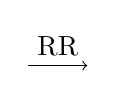
\begin{tikzpicture}
            \draw[->] (0,0) -- (0.75,0) node[midway, above] {RR};
        \end{tikzpicture}
        \hfill
        \begin{minipage}{0.45\textwidth}
            \centering
            \begin{forest} default tree style
                [60, red
                    [40
                        [20
                            [10]
                            [, phantom]
                        ]
                        [50
                            [45
                                [42]
                                [, phantom]
                            ]
                            [55
                                [52]
                                [56]
                            ]
                        ]
                    ]
                    [80
                        [70]
                        [90]
                    ]
                ]
            \end{forest}
        \end{minipage}
        
        \hfill
        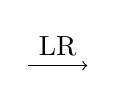
\begin{tikzpicture}
            \draw[->] (0,0) -- (0.75,0) node[midway, above] {LR};
        \end{tikzpicture}
        \hfill
        \begin{minipage}{0.60\textwidth}
            \centering
            \begin{forest} default tree style
                [50
                    [40
                        [20
                            [10]
                            [, phantom]
                        ]
                        [45
                            [42]
                            [, phantom]
                        ]
                    ]
                    [60
                        [55
                            [52]
                            [56]
                        ]
                        [80
                            [70]
                            [90]
                        ]
                    ]
                ]
            \end{forest}
        \end{minipage}
    \end{solution}

\end{questions}

\end{document}